\documentclass[12pt]{article}

\usepackage{sbc-template}
\usepackage[brazil]{babel}
\usepackage[utf8]{inputenc}
\usepackage[T1]{fontenc}
\usepackage{graphicx,url,amsmath,amssymb,booktabs,multirow}
\usepackage[hidelinks]{hyperref}
\graphicspath{{../figuras/}}

\newcommand{\nomeautor}{Cledson da Silva Araújo}
% Gerado por relatorio/gerar_numeros.py — não editar à mão.
\newcommand{\nNV}{1.560.938}
\newcommand{\nObitosSIM}{13.471}
\newcommand{\nPareados}{12.155}
\newcommand{\pctPareado}{90,2\%}
\newcommand{\pctPareadoMin}{88,5\%}
\newcommand{\pctPareadoMax}{91,6\%}
\newcommand{\tmnSIM}{8,63}
\newcommand{\tmnPareada}{7,79}
\newcommand{\nPassadas}{6}
\newcommand{\pctParesUmDois}{82\%}
\newcommand{\falsosUmDoisMax}{8\%}
\newcommand{\falsosMax}{31\%}
\newcommand{\falsosPonderado}{6\%}
\newcommand{\anoIni}{2017}
\newcommand{\anoFim}{2024}
\newcommand{\anoObFim}{2025}
\newcommand{\anoValid}{2023}
\newcommand{\anoAjFim}{2022}
\newcommand{\anoTeste}{2024}
\newcommand{\nAjuste}{1.221.071}
\newcommand{\obAjuste}{9.405}
\newcommand{\tmnAjuste}{7,70}
\newcommand{\nValid}{176.145}
\newcommand{\obValid}{1.444}
\newcommand{\tmnValid}{8,20}
\newcommand{\nTeste}{163.722}
\newcommand{\obTeste}{1.306}
\newcommand{\tmnTeste}{7,98}
\newcommand{\razaoEscol}{1,6}
\newcommand{\nVarsA}{28}
\newcommand{\nVarsB}{17}
\newcommand{\ALrAuroc}{0,963}
\newcommand{\ALrAurocIC}{0,963 (0,956--0,969)}
\newcommand{\ALrAuprc}{0,551}
\newcommand{\ALrAuprcIC}{0,551 (0,526--0,579)}
\newcommand{\ALrFum}{0,554}
\newcommand{\ALrFumIC}{0,554 (0,534--0,574)}
\newcommand{\ALrPrec}{0,534}
\newcommand{\ALrPrecIC}{0,534 (0,514--0,556)}
\newcommand{\ALrSens}{0,577}
\newcommand{\ALrSensIC}{0,577 (0,549--0,600)}
\newcommand{\ALrEspec}{0,996}
\newcommand{\ALrEspecIC}{0,996 (0,996--0,996)}
\newcommand{\ALrVpn}{0,997}
\newcommand{\ALrVpnIC}{0,997 (0,996--0,997)}
\newcommand{\ALrBrier}{0,0049}
\newcommand{\ALrBrierIC}{0,0049 (0,0047--0,0051)}
\newcommand{\ALrTop}{88\%}
\newcommand{\ALrOE}{0,93}
\newcommand{\AXgbAuroc}{0,964}
\newcommand{\AXgbAurocIC}{0,964 (0,958--0,970)}
\newcommand{\AXgbAuprc}{0,603}
\newcommand{\AXgbAuprcIC}{0,603 (0,577--0,628)}
\newcommand{\AXgbFum}{0,604}
\newcommand{\AXgbFumIC}{0,604 (0,583--0,625)}
\newcommand{\AXgbPrec}{0,597}
\newcommand{\AXgbPrecIC}{0,597 (0,576--0,620)}
\newcommand{\AXgbSens}{0,610}
\newcommand{\AXgbSensIC}{0,610 (0,583--0,636)}
\newcommand{\AXgbEspec}{0,997}
\newcommand{\AXgbEspecIC}{0,997 (0,996--0,997)}
\newcommand{\AXgbVpn}{0,997}
\newcommand{\AXgbVpnIC}{0,997 (0,997--0,997)}
\newcommand{\AXgbBrier}{0,0045}
\newcommand{\AXgbBrierIC}{0,0045 (0,0043--0,0047)}
\newcommand{\AXgbTop}{88\%}
\newcommand{\AXgbOE}{0,95}
\newcommand{\ALgbmAuroc}{0,964}
\newcommand{\ALgbmAurocIC}{0,964 (0,958--0,970)}
\newcommand{\ALgbmAuprc}{0,580}
\newcommand{\ALgbmAuprcIC}{0,580 (0,552--0,608)}
\newcommand{\ALgbmFum}{0,596}
\newcommand{\ALgbmFumIC}{0,596 (0,573--0,617)}
\newcommand{\ALgbmPrec}{0,610}
\newcommand{\ALgbmPrecIC}{0,610 (0,586--0,633)}
\newcommand{\ALgbmSens}{0,583}
\newcommand{\ALgbmSensIC}{0,583 (0,556--0,608)}
\newcommand{\ALgbmEspec}{0,997}
\newcommand{\ALgbmEspecIC}{0,997 (0,997--0,997)}
\newcommand{\ALgbmVpn}{0,997}
\newcommand{\ALgbmVpnIC}{0,997 (0,996--0,997)}
\newcommand{\ALgbmBrier}{0,0046}
\newcommand{\ALgbmBrierIC}{0,0046 (0,0044--0,0048)}
\newcommand{\ALgbmTop}{88\%}
\newcommand{\ALgbmOE}{0,94}
\newcommand{\BLrAuroc}{0,886}
\newcommand{\BLrAurocIC}{0,886 (0,874--0,896)}
\newcommand{\BLrAuprc}{0,366}
\newcommand{\BLrAuprcIC}{0,366 (0,338--0,394)}
\newcommand{\BLrFum}{0,450}
\newcommand{\BLrFumIC}{0,450 (0,429--0,471)}
\newcommand{\BLrPrec}{0,434}
\newcommand{\BLrPrecIC}{0,434 (0,411--0,455)}
\newcommand{\BLrSens}{0,467}
\newcommand{\BLrSensIC}{0,467 (0,442--0,492)}
\newcommand{\BLrEspec}{0,995}
\newcommand{\BLrEspecIC}{0,995 (0,995--0,995)}
\newcommand{\BLrVpn}{0,996}
\newcommand{\BLrVpnIC}{0,996 (0,996--0,996)}
\newcommand{\BLrBrier}{0,0059}
\newcommand{\BLrBrierIC}{0,0059 (0,0058--0,0061)}
\newcommand{\BLrTop}{71\%}
\newcommand{\BLrOE}{0,95}
\newcommand{\BXgbAuroc}{0,891}
\newcommand{\BXgbAurocIC}{0,891 (0,879--0,902)}
\newcommand{\BXgbAuprc}{0,390}
\newcommand{\BXgbAuprcIC}{0,390 (0,360--0,418)}
\newcommand{\BXgbFum}{0,454}
\newcommand{\BXgbFumIC}{0,454 (0,432--0,476)}
\newcommand{\BXgbPrec}{0,470}
\newcommand{\BXgbPrecIC}{0,470 (0,446--0,494)}
\newcommand{\BXgbSens}{0,440}
\newcommand{\BXgbSensIC}{0,440 (0,413--0,464)}
\newcommand{\BXgbEspec}{0,996}
\newcommand{\BXgbEspecIC}{0,996 (0,996--0,996)}
\newcommand{\BXgbVpn}{0,995}
\newcommand{\BXgbVpnIC}{0,995 (0,995--0,996)}
\newcommand{\BXgbBrier}{0,0059}
\newcommand{\BXgbBrierIC}{0,0059 (0,0057--0,0061)}
\newcommand{\BXgbTop}{71\%}
\newcommand{\BXgbOE}{0,96}
\newcommand{\BLgbmAuroc}{0,890}
\newcommand{\BLgbmAurocIC}{0,890 (0,879--0,901)}
\newcommand{\BLgbmAuprc}{0,396}
\newcommand{\BLgbmAuprcIC}{0,396 (0,367--0,424)}
\newcommand{\BLgbmFum}{0,457}
\newcommand{\BLgbmFumIC}{0,457 (0,435--0,481)}
\newcommand{\BLgbmPrec}{0,466}
\newcommand{\BLgbmPrecIC}{0,466 (0,441--0,490)}
\newcommand{\BLgbmSens}{0,448}
\newcommand{\BLgbmSensIC}{0,448 (0,423--0,474)}
\newcommand{\BLgbmEspec}{0,996}
\newcommand{\BLgbmEspecIC}{0,996 (0,996--0,996)}
\newcommand{\BLgbmVpn}{0,996}
\newcommand{\BLgbmVpnIC}{0,996 (0,995--0,996)}
\newcommand{\BLgbmBrier}{0,0059}
\newcommand{\BLgbmBrierIC}{0,0059 (0,0057--0,0060)}
\newcommand{\BLgbmTop}{71\%}
\newcommand{\BLgbmOE}{0,97}
\newcommand{\dAB}{0,074}
\newcommand{\dABIC}{0,064--0,084}
\newcommand{\dXLa}{0,001}
\newcommand{\dXLaIC}{-0,001--0,003}
\newcommand{\dXLb}{0,005}
\newcommand{\dXLbIC}{-0,000--0,011}
\newcommand{\dABprc}{0,214}
\newcommand{\dABprcIC}{0,191--0,241}
\newcommand{\dXLaprc}{0,052}
\newcommand{\dXLaprcIC}{0,040--0,066}
\newcommand{\dXLbprc}{0,024}
\newcommand{\dXLbprcIC}{0,011--0,041}
\newcommand{\oeBrutoA}{0,23}
\newcommand{\arvA}{247}
\newcommand{\profA}{5}
\newcommand{\lrA}{0,036}
\newcommand{\spwA}{11}
\newcommand{\sensAEstAuroc}{0,963}
\newcommand{\sensAEstAuprc}{0,601}
\newcommand{\sensAEstOE}{1,07}
\newcommand{\sensAEstDelta}{-0,0009 (-0,0020 a 0,0001)}
\newcommand{\sensAPiorAuroc}{0,963}
\newcommand{\sensAPiorAuprc}{0,599}
\newcommand{\sensAPiorOE}{1,16}
\newcommand{\sensAPiorDelta}{-0,0013 (-0,0029 a 0,0005)}
\newcommand{\calABruInt}{-2,456 (-2,526 a -2,387)}
\newcommand{\calABruInc}{1,058 (1,029 a 1,088)}
\newcommand{\calACalInt}{-0,082 (-0,154 a -0,011)}
\newcommand{\calACalInc}{1,009 (0,981 a 1,037)}
\newcommand{\nbAUm}{6,6}
\newcommand{\sinalAUm}{5,6\%}
\newcommand{\nbACinco}{5,5}
\newcommand{\sinalACinco}{2,3\%}
\newcommand{\nbAVinte}{4,1}
\newcommand{\sinalAVinte}{1,1\%}
\newcommand{\nbPositivoA}{sim}
\newcommand{\oeBrutoB}{0,17}
\newcommand{\arvB}{407}
\newcommand{\profB}{5}
\newcommand{\lrB}{0,036}
\newcommand{\spwB}{11}
\newcommand{\sensBEstAuroc}{0,891}
\newcommand{\sensBEstAuprc}{0,392}
\newcommand{\sensBEstOE}{1,11}
\newcommand{\sensBEstDelta}{0,0006 (-0,0015 a 0,0029)}
\newcommand{\sensBPiorAuroc}{0,892}
\newcommand{\sensBPiorAuprc}{0,391}
\newcommand{\sensBPiorOE}{1,16}
\newcommand{\sensBPiorDelta}{0,0013 (-0,0009 a 0,0034)}
\newcommand{\calBBruInt}{-2,410 (-2,473 a -2,347)}
\newcommand{\calBBruInc}{1,016 (0,990 a 1,043)}
\newcommand{\calBCalInt}{-0,060 (-0,124 a 0,004)}
\newcommand{\calBCalInc}{0,979 (0,954 a 1,005)}
\newcommand{\nbBUm}{5,3}
\newcommand{\sinalBUm}{7,0\%}
\newcommand{\nbBCinco}{4,0}
\newcommand{\sinalBCinco}{2,4\%}
\newcommand{\nbBVinte}{2,6}
\newcommand{\sinalBVinte}{0,9\%}
\newcommand{\nbPositivoB}{sim}
\newcommand{\driftLog}{0,035}
\newcommand{\posTreinoEstrito}{7.661}
\newcommand{\nNaoPareados}{1.316}
\newcommand{\parPesoAus}{0,8}
\newcommand{\nparPesoAus}{26,8}
\newcommand{\parSemAus}{4,8}
\newcommand{\nparSemAus}{31,5}
\newcommand{\parIdAus}{2,1}
\newcommand{\nparIdAus}{32,2}
\newcommand{\parCap}{35,0}
\newcommand{\nparCap}{19,6}
\newcommand{\parHosp}{98,2}
\newcommand{\nparHosp}{90,2}
\newcommand{\parPesoMed}{1100}
\newcommand{\nparPesoMed}{1400}
\newcommand{\linkCap}{94,3\%}
\newcommand{\linkInt}{88,2\%}
\newcommand{\linkRacaMin}{89,4\%}
\newcommand{\linkRacaMax}{90,6\%}
\newcommand{\linkPesoAus}{20,7\%}
\newcommand{\pctVerdadeiros}{85\%}
\newcommand{\vifFilhos}{20}
\newcommand{\vifGest}{22}
\newcommand{\vifPartos}{4,5}
\newcommand{\vifOutrosMax}{4,6}
\newcommand{\ausCons}{19,7}
\newcommand{\preCons}{7,5}
\newcommand{\pctAusCons}{2,2}
\newcommand{\ausPai}{8,8}
\newcommand{\prePai}{6,6}
\newcommand{\pctAusPai}{54,7}
\newcommand{\ausSem}{13,4}
\newcommand{\preSem}{7,7}
\newcommand{\pctAusSem}{1,1}
\newcommand{\ausApg}{27,6}
\newcommand{\preApg}{7,6}
\newcommand{\pctAusApg}{1,1}
\newcommand{\pctMult}{2,3}
\newcommand{\pctObMult}{10,2}
\newcommand{\aurocUnicosA}{0,963}
\newcommand{\aurocUnicosB}{0,882}
\newcommand{\repo}{https://github.com/CledsonSilvaAraujo/mortalidade-neonatal-rj}
\newcommand{\tempoMin}{41}
\newcommand{\subAAurocMin}{0,950}
\newcommand{\subAAurocMax}{0,980}
\newcommand{\subAFundAuroc}{0,950 (0,932--0,965)}
\newcommand{\subAFundOE}{0,99 (0,90--1,08)}
\newcommand{\subASupAuroc}{0,980 (0,970--0,989)}
\newcommand{\subASupOE}{0,92 (0,84--1,00)}
\newcommand{\subABrancaAuroc}{0,976 (0,966--0,983)}
\newcommand{\subABrancaOE}{0,98 (0,91--1,05)}
\newcommand{\subAPretaAuroc}{0,962 (0,946--0,976)}
\newcommand{\subAPretaOE}{0,92 (0,84--1,01)}
\newcommand{\subACapAuroc}{0,966 (0,954--0,976)}
\newcommand{\subACapOE}{0,91 (0,85--0,97)}
\newcommand{\subAIntAuroc}{0,963 (0,955--0,970)}
\newcommand{\subAIntOE}{0,98 (0,93--1,02)}
\newcommand{\subBAurocMin}{0,875}
\newcommand{\subBAurocMax}{0,906}
\newcommand{\subBFundAuroc}{0,875 (0,846--0,897)}
\newcommand{\subBFundOE}{0,99 (0,90--1,09)}
\newcommand{\subBSupAuroc}{0,902 (0,872--0,928)}
\newcommand{\subBSupOE}{0,94 (0,85--1,05)}
\newcommand{\subBBrancaAuroc}{0,898 (0,877--0,919)}
\newcommand{\subBBrancaOE}{1,02 (0,94--1,11)}
\newcommand{\subBPretaAuroc}{0,906 (0,878--0,929)}
\newcommand{\subBPretaOE}{0,94 (0,85--1,03)}
\newcommand{\subBCapAuroc}{0,885 (0,863--0,906)}
\newcommand{\subBCapOE}{0,94 (0,87--1,02)}
\newcommand{\subBIntAuroc}{0,894 (0,880--0,907)}
\newcommand{\subBIntOE}{0,97 (0,91--1,02)}
\newcommand{\shapTopA}{peso ao nascer, Apgar 5º min, Apgar 1º min, semanas de gestação, anomalia congênita}
\newcommand{\shapTopB}{semanas de gestação, consultas de pré-natal, escolaridade da mãe, apresentação, raça/cor da mãe}
\newcommand{\compTreinoCap}{94,3\%}
\newcommand{\compTesteCap}{94,6\%}
\newcommand{\oeLinkCap}{1,003}
\newcommand{\compDifCap}{0,3}
\newcommand{\oeRegACapBru}{0,22}
\newcommand{\oeRegACapCal}{0,91}
\newcommand{\oeRegBCapBru}{0,17}
\newcommand{\oeRegBCapCal}{0,94}
\newcommand{\compTreinoInt}{88,0\%}
\newcommand{\compTesteInt}{89,6\%}
\newcommand{\oeLinkInt}{1,018}
\newcommand{\compDifInt}{1,6}
\newcommand{\oeRegAIntBru}{0,24}
\newcommand{\oeRegAIntCal}{0,98}
\newcommand{\oeRegBIntBru}{0,17}
\newcommand{\oeRegBIntCal}{0,97}
\newcommand{\testeEstrAAuroc}{0,965}
\newcommand{\testeZeroAAuroc}{0,964}
\newcommand{\nbADois}{6,2}
\newcommand{\nbADez}{4,9}
\newcommand{\testeEstrBAuroc}{0,890}
\newcommand{\testeZeroBAuroc}{0,890}
\newcommand{\nbBDois}{4,7}
\newcommand{\nbBDez}{3,3}
\newcommand{\antABrancaOE}{1,08}
\newcommand{\antAIntOE}{1,05}
\newcommand{\antBBrancaOE}{1,15}
\newcommand{\antBIntOE}{1,08}
\newcommand{\anoTesteAnt}{2023}
\newcommand{\tmnPesoMuitoBaixo}{285}
\newcommand{\tmnPesoNormal}{1,9}
\newcommand{\tmnIgMuitoPrematuro}{262}
\newcommand{\tmnIgTermo}{2,0}
\newcommand{\tmnApgarBaixo}{306}
\newcommand{\xaiSpearA}{0,90}
\newcommand{\xaiTopA}{4}
\newcommand{\xaiMetadesA}{0,999}
\newcommand{\xaiSensA}{3,0\%}
\newcommand{\xaiAditA}{7\times 10^{-6}}
\newcommand{\xaiSpearB}{0,98}
\newcommand{\xaiTopB}{5}
\newcommand{\xaiMetadesB}{0,998}
\newcommand{\xaiSensB}{7,9\%}
\newcommand{\xaiAditB}{6\times 10^{-6}}
\newcommand{\xaiBrancaB}{-0,11}
\newcommand{\xaiPretaB}{0,06}
\newcommand{\xaiEscBaixaB}{0,33}
\newcommand{\xaiEscSupB}{-0,27}
\newcommand{\xaiBase}{6,18\%}
\newcommand{\xaiFnProb}{4,4\%}
\newcommand{\xaiFpProb}{100,0\%}
\newcommand{\xaiVpPeso}{670~g}
\newcommand{\xaiVpApgarUm}{1}
\newcommand{\xaiVpApgarCinco}{1}
\newcommand{\xaiVpSem}{22}
\newcommand{\xaiVpAnom}{com anomalia}
\newcommand{\xaiVpProb}{100,0\%}
\newcommand{\xaiFnPeso}{3.450~g}
\newcommand{\xaiFnApgarUm}{7}
\newcommand{\xaiFnApgarCinco}{8}
\newcommand{\xaiFnSem}{39}
\newcommand{\xaiFnAnom}{com anomalia}
\newcommand{\xaiFpPeso}{385~g}
\newcommand{\xaiFpApgarUm}{1}
\newcommand{\xaiFpApgarCinco}{1}
\newcommand{\xaiFpSem}{21}
\newcommand{\nNVEn}{1,560,938}
\newcommand{\nObitosSIMEn}{13,471}
\newcommand{\pctPareadoEn}{90.2\%}
\newcommand{\pctVerdadeirosEn}{85\%}
\newcommand{\AXgbAurocICEn}{0.964 (95\% CI 0.958--0.970)}
\newcommand{\AXgbAuprcEn}{0.603}
\newcommand{\AXgbTopEn}{88\%}
\newcommand{\BXgbAurocEn}{0.891}
\newcommand{\parUm}{6.043}
\newcommand{\falsosUm}{0\%}
\newcommand{\parDois}{3.917}
\newcommand{\falsosDois}{6--8\%}
\newcommand{\parTres}{846}
\newcommand{\falsosTres}{17--31\%}
\newcommand{\parQuatro}{479}
\newcommand{\falsosQuatro}{12--16\%}
\newcommand{\parCinco}{547}
\newcommand{\falsosCinco}{12--14\%}
\newcommand{\parSeis}{323}
\newcommand{\falsosSeis}{21--22\%}
\newcommand{\prevPareada}{0,78\%}
\newcommand{\hpALr}{0,036}
\newcommand{\hpAMcw}{1,57}
\newcommand{\hpASub}{0,93}
\newcommand{\hpACol}{0,77}
\newcommand{\hpALam}{0,021}
\newcommand{\hpAAlp}{0,002}
\newcommand{\hpAGam}{0,014}
\newcommand{\hpASpw}{11,35}
\newcommand{\hpAProf}{5}
\newcommand{\hpAArv}{247}
\newcommand{\hpBLr}{0,036}
\newcommand{\hpBMcw}{1,57}
\newcommand{\hpBSub}{0,93}
\newcommand{\hpBCol}{0,77}
\newcommand{\hpBLam}{0,021}
\newcommand{\hpBAlp}{0,002}
\newcommand{\hpBGam}{0,014}
\newcommand{\hpBSpw}{11,35}
\newcommand{\hpBProf}{5}
\newcommand{\hpBArv}{407}
\newcommand{\pesoEscolhido}{√(n₀/n₁)}
\newcommand{\tabLinkage}{\begin{tabular}{clrrr}
\toprule
& Chave & Pares & \multicolumn{2}{c}{Falsos pares estimados} \\
\cmidrule(lr){4-5}
& & & Escol. mãe & Perdas fetais \\
\midrule
1 & data + sexo + mun. + peso + id. mãe + sem. gest. + gravidez + parto & 6.043 & 0\% & 0\% \\
2 & data + sexo + mun. + peso + id. mãe & 3.917 & 6\% & 8\% \\
3 & data + sexo + mun. + peso + estab. & 846 & 31\% & 17\% \\
4 & data + sexo + peso + id. mãe & 479 & 12\% & 16\% \\
5 & data + sexo + mun. + id. mãe + sem. gest. & 547 & 14\% & 12\% \\
6 & data + sexo + mun. + estab. + id. mãe & 323 & 21\% & 22\% \\
\bottomrule
\end{tabular}}
\newcommand{\tabMetricas}{\begin{tabular}{llcccccc}
\toprule
Conj. & Modelo & AUROC & AUPRC & F1 & Precisão & Sensib. & Top 5\% \\
\midrule
A & LR & 0,963 (0,956--0,969) & 0,551 (0,526--0,579) & 0,554 & 0,534 & 0,577 & 88\% \\
A & XGBoost & \textbf{0,964 (0,958--0,970)} & \textbf{0,603 (0,577--0,628)} & 0,604 & 0,597 & 0,610 & 88\% \\
A & LightGBM & 0,964 (0,958--0,970) & 0,580 (0,552--0,608) & 0,596 & 0,610 & 0,583 & 88\% \\
\midrule
B & LR & 0,886 (0,874--0,896) & 0,366 (0,338--0,394) & 0,450 & 0,434 & 0,467 & 71\% \\
B & XGBoost & \textbf{0,891 (0,879--0,902)} & \textbf{0,390 (0,360--0,418)} & 0,454 & 0,470 & 0,440 & 71\% \\
B & LightGBM & 0,890 (0,879--0,901) & 0,396 (0,367--0,424) & 0,457 & 0,466 & 0,448 & 71\% \\
\midrule
\multicolumn{2}{l}{Batista et al. (SP)} & 0,971 & 0,586 & 0,548 & 0,729 & 0,440 & $>$90\% \\
\bottomrule
\end{tabular}}
\newcommand{\tabDescritiva}{\begin{tabular}{llrrr}
\toprule
Variável & Categoria & NV & Óbitos & TMN (‰) \\
\midrule
Peso ao nascer & $<$ 1.500 g & 25.466 & 7.268 & 285,4 \\
 & 1.500–2.499 g & 123.814 & 2.136 & 17,3 \\
 & 2.500–3.999 g & 1.335.475 & 2.600 & 1,9 \\
 & $\geq$ 4.000 g & 76.156 & 151 & 2,0 \\
\addlinespace
Idade gestacional & $<$ 32 sem & 26.081 & 6.836 & 262,1 \\
 & 32–36 sem & 150.762 & 2.306 & 15,3 \\
 & 37–41 sem & 1.342.386 & 2.726 & 2,0 \\
 & $\geq$ 42 sem & 23.810 & 48 & 2,0 \\
\addlinespace
Escolaridade da mãe & Fund. incompleto ou menos & 362.104 & 3.404 & 9,4 \\
 & Médio & 834.071 & 6.567 & 7,9 \\
 & Superior & 339.602 & 1.960 & 5,8 \\
\bottomrule
\end{tabular}}
\newcommand{\tabHiper}{\begin{tabular}{lrr}
\toprule
Hiperparâmetro & A · completo & B · pré-parto \\
\midrule
\texttt{learning\_rate} & 0,036 & 0,036 \\
\texttt{max\_depth} & 5 & 5 \\
\texttt{min\_child\_weight} & 1,573 & 1,573 \\
\texttt{subsample} & 0,932 & 0,932 \\
\texttt{colsample\_bytree} & 0,774 & 0,774 \\
\texttt{reg\_lambda} & 0,021 & 0,021 \\
\texttt{reg\_alpha} & 0,002 & 0,002 \\
\texttt{gamma} & 0,014 & 0,014 \\
\texttt{scale\_pos\_weight} & 11,350 & 11,350 \\
\texttt{n\_arvores} & 247 & 407 \\
\bottomrule
\end{tabular}}
\newcommand{\tabVies}{\begin{tabular}{lrr}
\toprule
Característica (na DO) & Pareados & Não pareados \\
\midrule
n & 12.155 & 1.316 \\
Peso ausente (\%) & 0,8 & 26,8 \\
Semanas ausentes (\%) & 4,8 & 31,5 \\
Idade da mãe ausente (\%) & 2,1 & 32,2 \\
Peso mediano (g) & 1.100 & 1.400 \\
Peso $<$ 1.500 g (\%) & 60,2 & 52,1 \\
Óbito no 1º dia (\%) & 26,5 & 31,6 \\
Residente na capital (\%) & 35,0 & 19,6 \\
Óbito em hospital (\%) & 98,2 & 90,2 \\
\bottomrule
\end{tabular}}
\newcommand{\tabSens}{\begin{tabular}{llcccc}
\toprule
Conj. & Rótulos no treino & AUROC & AUPRC & O/E & $\Delta$AUROC (IC 95\%) \\
\midrule
A & principal & 0,964 & 0,603 & 0,95 & -- \\
A & estrito (sem passadas 3--6) & 0,963 & 0,601 & 1,07 & -0,0009 (-0,0020 a 0,0001) \\
A & pior caso (passadas 3--6 = 0) & 0,963 & 0,599 & 1,16 & -0,0013 (-0,0029 a 0,0005) \\
\midrule
B & principal & 0,891 & 0,390 & 0,96 & -- \\
B & estrito (sem passadas 3--6) & 0,891 & 0,392 & 1,11 & 0,0006 (-0,0015 a 0,0029) \\
B & pior caso (passadas 3--6 = 0) & 0,892 & 0,391 & 1,16 & 0,0013 (-0,0009 a 0,0034) \\
\bottomrule
\end{tabular}}
\newcommand{\tabCompletude}{\begin{tabular}{lccccc}
\toprule
Região & Pareamento treino & Pareamento 2024 & O/E esperado & O/E A & O/E B \\
& (2017--2023) & & só pelo linkage & (recalibr.) & (recalibr.) \\
\midrule
Capital & 94,3\% & 94,6\% & 1,003 & 0,91 & 0,94 \\
Interior & 88,0\% & 89,6\% & 1,018 & 0,98 & 0,97 \\
\bottomrule
\end{tabular}}


\sloppy

\title{Predição de mortalidade neonatal no Rio de Janeiro\\
com dados abertos: linkage SINASC $\times$ SIM\\
sem identificadores e aprendizado de máquina}

\author{\nomeautor\inst{1}}

\address{Instituto de Computação -- Universidade Federal Fluminense (UFF)\\
  Niterói -- RJ -- Brasil}

\begin{document}

\maketitle

\begin{abstract}
Batista et al. (2021) predicted neonatal death in São Paulo with XGBoost (AUROC 0.971), but relied on identified records linked by the city. We reproduce and extend their study for the state of Rio de Janeiro using only public DATASUS microdata. The data cover \nNV{} live births in 2017--2023. Because the public files have no identifiers, we linked births and deaths with cascaded composite keys and matched \pctPareado{} of the \nObitosSIM{} neonatal deaths, a rate comparable to what identified data achieve. Models were trained on 2017--2021, tuned and recalibrated on 2022, and tested once on 2023. With all birth-certificate variables, XGBoost reached an AUROC of \AXgbAurocIC{} and an AUPRC of \AXgbAuprc{}, and the 5\% highest-risk births held \AXgbTop{} of deaths. A model restricted to information available at admission for delivery reached an AUROC of \BXgbAuroc{}, with good calibration. The full model performed similarly across maternal race, education and region; the pre-delivery model underestimated risk for births to white mothers and outside the capital.
\end{abstract}

\begin{resumo}
Batista et al. (2021) previram o óbito neonatal em São Paulo com XGBoost e obtiveram AUROC de 0,971, mas usaram registros identificados, pareados pela prefeitura. Este trabalho reproduz e estende o estudo para o estado do Rio de Janeiro usando apenas microdados públicos do DATASUS. Os dados cobrem \nNV{} nascidos vivos entre 2017 e 2023. Como os arquivos públicos não têm identificadores, os nascimentos foram pareados aos óbitos por chaves compostas em cascata. Foram pareados \pctPareado{} dos \nObitosSIM{} óbitos neonatais, taxa comparável à obtida com dados identificados. Os modelos foram treinados em 2017--2021, ajustados e recalibrados em 2022 e testados uma única vez em 2023. Com todas as variáveis da Declaração de Nascido Vivo, o XGBoost atingiu AUROC de \AXgbAurocIC{} e AUPRC de \AXgbAuprc{}; os 5\% de maior risco concentraram \AXgbTop{} dos óbitos. Um modelo restrito ao que se sabe na admissão para o parto atingiu AUROC de \BXgbAuroc{}, com boa calibração. O modelo completo teve desempenho semelhante entre os grupos de raça/cor e de escolaridade da mãe e entre capital e interior. O modelo pré-parto subestimou o risco para filhos de mães brancas e para residentes no interior.
\end{resumo}

% ---------------------------------------------------------------------------
\section{Introdução}

O período neonatal (0 a 27 dias de vida) concentra a maior parte dos óbitos infantis no Brasil, e boa parte deles é considerada evitável por atenção adequada à gestação, ao parto e ao recém-nascido. No estado do Rio de Janeiro, a taxa de mortalidade neonatal (TMN) entre 2017 e 2023 foi de \tmnSIM{} óbitos por mil nascidos vivos, segundo o Sistema de Informações sobre Mortalidade (SIM).

A Declaração de Nascido Vivo (DN) é preenchida para todo nascimento e alimenta o Sistema de Informações sobre Nascidos Vivos (SINASC). Um escore de risco calculado a partir dela poderia apoiar decisões como a priorização de leitos de UTI neonatal, o transporte inter-hospitalar e a visita domiciliar na primeira semana. Batista et al.~\cite{batista2021} mostraram que isso é viável: com as variáveis da DN do município de São Paulo, o XGBoost atingiu AUROC de 0,971.

O estudo, porém, deixa três lacunas:
\begin{itemize}
  \item usa dados identificados, que não estão disponíveis para terceiros;
  \item depende de variáveis que só existem depois do parto (Apgar, peso);
  \item não avalia calibração nem desempenho por subgrupo, lacunas também apontadas na revisão sistemática de \cite{mangold2021}.
\end{itemize}

Este trabalho responde a três perguntas:
\begin{enumerate}
  \item O desempenho do artigo se reproduz no estado do RJ usando apenas microdados públicos, que não têm identificadores? (H1: AUROC $\geq$ 0,95.)
  \item Quanto se perde com um modelo que usa só o que se sabe na admissão para o parto? (H2: queda substancial, com o modelo ainda útil para triagem.)
  \item O modelo é calibrado e funciona igualmente por raça/cor e escolaridade da mãe e entre capital e interior? (H3: pior nos subgrupos de menor escolaridade.)
\end{enumerate}

% ---------------------------------------------------------------------------
\section{Trabalhos relacionados}

\textbf{Artigo de referência.} \cite{batista2021} fizeram o linkage probabilístico de 1.202.843 nascimentos do município de São Paulo (2012--2017) com os registros de óbito, identificando 7.282 óbitos neonatais.
\begin{itemize}
  \item Foram usadas as 23 variáveis da DN para treinar cinco algoritmos: regressão logística, rede neural, XGBoost, LightGBM e CatBoost.
  \item Os hiperparâmetros foram escolhidos por otimização bayesiana com validação cruzada de 10 \textit{folds}.
  \item O treino usou 2012--2016 e o teste, 2017.
  \item O XGBoost teve o melhor desempenho: AUROC 0,971, AUPRC 0,586, F1 0,548, precisão 0,729 e sensibilidade 0,440.
  \item Os 5\% de maior risco concentraram mais de 90\% dos óbitos.
  \item Pelos valores SHAP, as variáveis mais importantes foram o Apgar no 5º e no 1º minuto, o peso ao nascer, a anomalia congênita e a idade gestacional.
\end{itemize}

\textbf{Modelos de mortalidade neonatal.} A revisão sistemática de \cite{mangold2021} reuniu 11 estudos, com 1,26 milhão de neonatos, e encontrou AUROC entre 0,58 e 0,97. Peso, idade gestacional, Apgar e gemelaridade foram os preditores mais comuns. Apenas 45\% dos estudos reportaram curvas de calibração, e 18\% fizeram validação externa.

\textbf{Linkage SIM $\times$ SINASC.} \cite{maia2017} parearam 90,8\% dos óbitos infantis das 27 capitais brasileiras aos respectivos nascimentos, combinando etapas determinísticas e probabilísticas sobre dados identificados. Nessas condições, o pareamento foi maior para óbitos neonatais do que para pós-neonatais.

% ---------------------------------------------------------------------------
\section{Dados}

\subsection{Fontes}

Foram usados os microdados públicos do SINASC (arquivos \texttt{DNRJ2017}--\texttt{DNRJ2023}) e do SIM (\texttt{DORJ2017}--\texttt{DORJ2024}) por residência no estado do RJ, obtidos no FTP do DATASUS sem cadastro \cite{datasus}. O SIM vai até 2024 para incluir os óbitos de quem nasceu no fim de 2023.

O desfecho é o óbito não fetal com 0 a 27 dias completos de vida, calculados pela diferença entre a data do óbito e a data de nascimento. Os arquivos somam \nNV{} nascidos vivos e \nObitosSIM{} óbitos neonatais.

\subsection{Linkage sem identificadores}

Os arquivos públicos não trazem o número da DN, o nome da mãe nem o endereço. No entanto, a Declaração de Óbito de menores de 1 ano repete dados do nascimento: data, sexo, peso, idade da mãe, semanas de gestação, tipo de gravidez e de parto. Além disso, o estabelecimento do óbito do neonato costuma ser o hospital onde ele nasceu.

Cada óbito foi pareado a um nascido vivo por concordância exata em \nPassadas{} chaves compostas aplicadas em cascata (Tabela~\ref{tab:linkage}). As chaves vão da mais restritiva à mais tolerante a campos ausentes. Em cada passada, uma chave só é aceita se for única entre os nascidos ainda não pareados e entre os óbitos ainda não pareados (pares 1:1).

Duas chaves adicionais foram testadas e descartadas por excesso estimado de falsos pares: data + sexo + município + peso, e data + sexo + município + estabelecimento. A segunda pareia neonatos transferidos com outro recém-nascido do hospital onde morreram.

\textbf{Estimativa de falsos pares.} Um campo que nunca entra nas chaves concorda nos pares verdadeiros com uma frequência $c_{\text{verd}}$ (menor que 100\%, por erros de registro) e nos pares falsos com a frequência do acaso, $c_{\text{acaso}}$. Se a passada $k$ tem uma fração $f_k$ de falsos pares, a concordância observada é
\begin{equation}
c_k = (1-f_k)\,c_{\text{verd}} + f_k\,c_{\text{acaso}}
\quad\Rightarrow\quad
f_k = \frac{c_{\text{verd}} - c_k}{c_{\text{verd}} - c_{\text{acaso}}}.
\end{equation}
Na estimativa:
\begin{itemize}
  \item $c_{\text{verd}}$ vem da passada 1, a chave completa;
  \item $c_{\text{acaso}}$ vem de pares sorteados com a mesma data de nascimento e o mesmo sexo;
  \item os campos de conferência são a escolaridade da mãe e o número de perdas fetais anteriores.
\end{itemize}

\begin{table}[ht]
\centering
\caption{Chaves do linkage, número de pares e fração estimada de falsos pares.}
\label{tab:linkage}
\small
\tabLinkage
\end{table}

\subsection{Preparação}

\textbf{Variáveis.} São 28 variáveis da DN:
\begin{itemize}
  \item 13 numéricas: idade da mãe e do pai, histórico obstétrico, semanas de gestação, consultas e mês de início do pré-natal, Apgar e peso;
  \item 14 categóricas, entre elas estado civil, escolaridade e raça/cor da mãe, tipo de gravidez e de parto, sexo, anomalia congênita, apresentação, indução, cesárea antes do trabalho de parto, grupo de Robson e índice de Kotelchuck;
  \item um indicador de residência na capital.
\end{itemize}

\textbf{Limpeza.}
\begin{itemize}
  \item Nas variáveis numéricas, os códigos de ``ignorado'' (99, ou 9999 no peso) viram ausentes.
  \item Nas categóricas, o ``9'' e o campo vazio viram categorias próprias, porque o não preenchimento da DN também informa sobre a assistência.
  \item A exclusão do artigo (idade gestacional fora de 15--45 semanas) não removeu nenhum registro, porque o SINASC já valida esse campo.
\end{itemize}

A Tabela~\ref{tab:desc} mostra a TMN pelos principais fatores. O gradiente é muito forte por peso e idade gestacional, e a TMN é \razaoEscol{} vezes maior entre filhos de mães com fundamental incompleto do que entre filhos de mães com ensino superior.

\begin{table}[ht]
\centering
\caption{Taxa de mortalidade neonatal (TMN, por mil nascidos vivos) na base pareada, 2017--2023.}
\label{tab:desc}
\small
\tabDescritiva
\end{table}

% ---------------------------------------------------------------------------
\section{Métodos}

\subsection{Conjuntos de variáveis}

\textbf{(A) Completo}: as \nVarsA{} variáveis descritas acima, que reproduzem o artigo.

\textbf{(B) Pré-parto}: \nVarsB{} variáveis conhecidas na admissão para o parto:
\begin{itemize}
  \item dados da mãe e do pai;
  \item histórico obstétrico;
  \item idade gestacional;
  \item tipo de gravidez e apresentação;
  \item consultas e início do pré-natal;
  \item índice de Kotelchuck;
  \item residência na capital.
\end{itemize}
Saem do conjunto B o Apgar, o peso, a anomalia congênita, o sexo, o local e o tipo de parto, a indução, a cesárea antes do trabalho de parto, quem assistiu o parto e o grupo de Robson. O grupo de Robson sai porque usa o início do trabalho de parto.

\subsection{Modelos}

\textbf{Regressão logística} (linha de base interpretável):
\begin{equation}
P(y=1\mid\mathbf{x}) = \sigma(\beta_0 + \boldsymbol\beta^\top\mathbf{x}), \qquad \sigma(z) = \frac{1}{1+e^{-z}}.
\end{equation}
O modelo usa penalização L2, com $C \in \{0{,}01;\ 0{,}1;\ 1\}$ escolhido na validação, e pesos de classe balanceados. Antes do ajuste há imputação pela mediana com indicador de ausência, padronização e \textit{one-hot}, todos ajustados só no treino.

\textbf{XGBoost} \cite{chen2016} \textbf{e LightGBM} \cite{ke2017}: o escore é uma soma de $K$ árvores de regressão,
\begin{equation}
F(\mathbf{x}) = \sum_{k=1}^{K} f_k(\mathbf{x}), \qquad P(y=1\mid\mathbf{x}) = \sigma(F(\mathbf{x})),
\end{equation}
ajustadas em sequência. A árvore $f_k$ minimiza a expansão de segunda ordem da log-loss mais a regularização $\Omega(f) = \gamma T + \tfrac{1}{2}\lambda\lVert w\rVert^2 + \alpha\lVert w\rVert_1$, com $T$ folhas e pesos $w$. As variáveis categóricas e os ausentes são tratados de forma nativa.

\textbf{Complexidade.}
\begin{itemize}
  \item Com histogramas, o ajuste custa $O(K\cdot n\cdot d)$ ($n$ registros, $d$ variáveis), e a predição custa $O(K\cdot\text{profundidade})$ por registro.
  \item A regressão logística custa $O(n\cdot d')$ por iteração do L-BFGS, com $d'$ colunas após o \textit{one-hot}.
  \item O experimento completo levou \tempoMin{} minutos em 32 núcleos.
\end{itemize}

\subsection{Validação}

A validação é temporal, como no artigo:
\begin{itemize}
  \item \textbf{ajuste} em 2017--2021 (\nAjuste{} nascidos vivos, \obAjuste{} óbitos);
  \item \textbf{validação} em 2022 (\nValid{}, \obValid{});
  \item \textbf{teste} em 2023 (\nTeste{}, \obTeste{}), usado uma única vez.
\end{itemize}

Na validação:
\begin{itemize}
  \item a busca bayesiana de hiperparâmetros (TPE, Optuna \cite{akiba2019}) maximizou a AUPRC, com 15 tentativas para o XGBoost e 10 para o LightGBM e \textit{early stopping} de 50 árvores;
  \item o peso da classe positiva foi tratado como hiperparâmetro (nenhum, $\sqrt{n_0/n_1}$ ou $n_0/n_1$), e a busca escolheu ``nenhum'' nos dois conjuntos;
  \item uma regressão isotônica recalibrou as probabilidades;
  \item o limiar de classificação foi o que maximiza o F1.
\end{itemize}
A Tabela~\ref{tab:hiper} lista os hiperparâmetros finais do XGBoost.

\begin{table}[ht]
\centering
\caption{Hiperparâmetros finais do XGBoost (número de árvores definido pelo \textit{early stopping}).}
\label{tab:hiper}
\small
\tabHiper
\end{table}

\subsection{Medidas de desempenho}

As métricas se dividem em dois grupos:
\begin{itemize}
  \item \textbf{Discriminação:} AUROC, AUPRC e fração dos óbitos entre os 5\% de maior risco, a métrica que permite comparar com o artigo.
  \item \textbf{Calibração e decisão:} escore de Brier, razão observado/esperado (O/E) e as métricas no limiar (F1, precisão, sensibilidade, especificidade e VPN).
\end{itemize}

A AUPRC é a métrica principal porque a prevalência é de $\approx$0,8\%. A isotônica é monótona, mas é uma função em degraus e cria empates. Por isso, a discriminação é medida pelo escore bruto do modelo, e o restante pela probabilidade recalibrada.

Os intervalos de confiança de 95\% vêm de 500 reamostras bootstrap estratificadas por desfecho. As diferenças entre modelos ($\Delta$AUROC e $\Delta$AUPRC) usam bootstrap pareado. A interpretação usa valores SHAP \cite{lundberg2017} (\textit{TreeExplainer}) numa amostra de 20.000 nascimentos de 2023.

Como análise de sensibilidade, o XGBoost foi refeito sem os pares das passadas 3 a 6 do linkage.

% ---------------------------------------------------------------------------
\section{Resultados}

\subsection{Linkage}

Foram pareados \nPareados{} dos \nObitosSIM{} óbitos neonatais (\pctPareado{}), com variação de \pctPareadoMin{} a \pctPareadoMax{} entre os anos (Figura~\ref{fig:linkage}). As passadas 1 e 2 respondem por \pctParesUmDois{} dos pares e têm até \falsosUmDoisMax{} de falsos pares estimados. As passadas tolerantes chegam a \falsosMax{}, e a média ponderada é de \falsosPonderado{}. A TMN da base pareada é de \tmnPareada{}‰, contra \tmnSIM{}‰ no SIM.

\begin{figure}[ht]
\centering
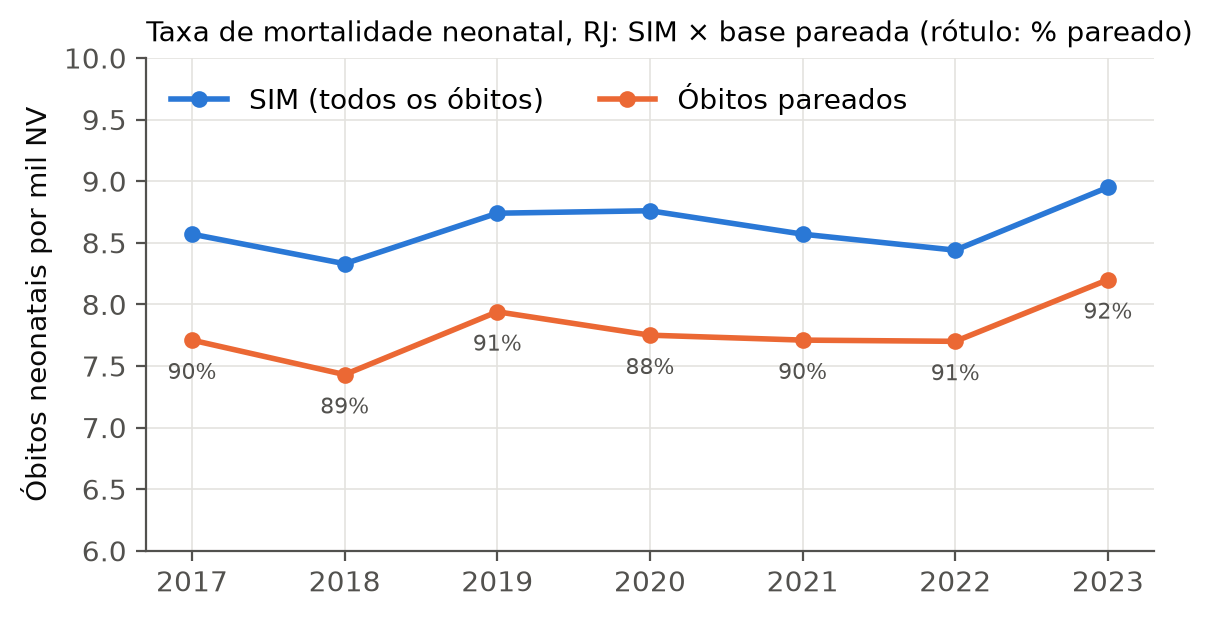
\includegraphics[width=0.72\textwidth]{linkage_por_ano.png}
\caption{TMN no SIM e na base pareada por ano de nascimento; os rótulos indicam o percentual de óbitos pareados.}
\label{fig:linkage}
\end{figure}

\subsection{Desempenho}

A Tabela~\ref{tab:metricas} resume o teste de 2023. Com o conjunto completo (A):
\begin{itemize}
  \item o XGBoost atingiu AUROC de \AXgbAurocIC{} e AUPRC de \AXgbAuprcIC{};
  \item os 5\% de maior risco concentraram \AXgbTop{} dos óbitos;
  \item no limiar escolhido em 2022, F1 = \AXgbFum{}, precisão = \AXgbPrec{}, sensibilidade = \AXgbSens{} e VPN = \AXgbVpn{}.
\end{itemize}

O ganho do XGBoost sobre a regressão logística foi pequeno. Em AUROC, $\Delta$ = \dXLa{} (IC \dXLaIC{}), com limite inferior praticamente nulo. Em AUPRC, o ganho foi mais claro: $\Delta$ = \dXLaprc{} (IC \dXLaprcIC{}). O LightGBM ficou praticamente empatado com o XGBoost. A Figura~\ref{fig:roc} mostra as curvas ROC e precisão--sensibilidade.

\begin{table}[ht]
\centering
\caption{Desempenho no teste de 2023 (IC 95\% por bootstrap). AUROC, AUPRC e top 5\% vêm do escore bruto; F1, precisão e sensibilidade, do limiar escolhido em 2022.}
\label{tab:metricas}
\small
\setlength{\tabcolsep}{4pt}
\tabMetricas
\end{table}

\begin{figure}[ht]
\centering
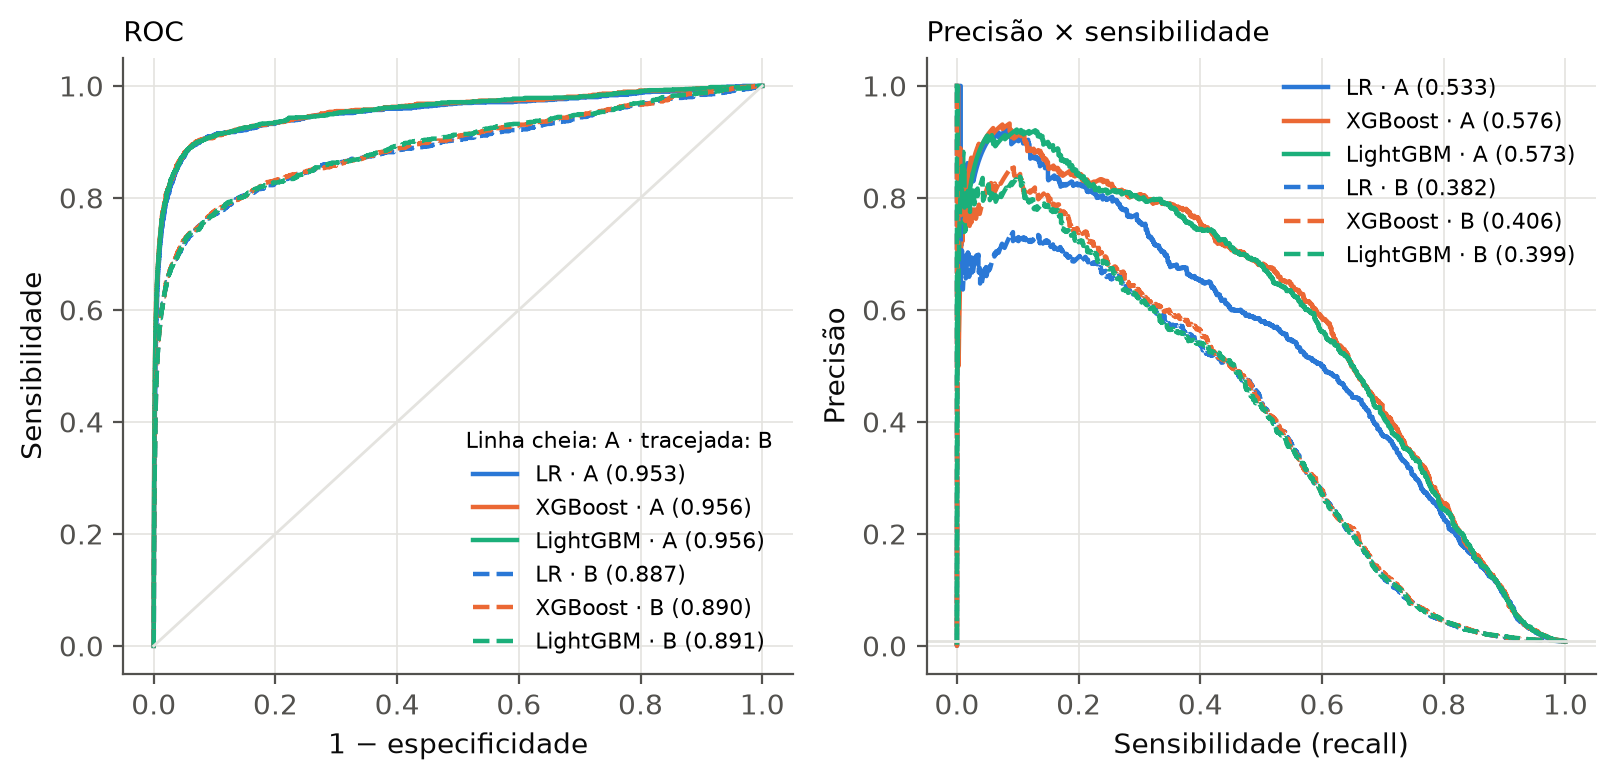
\includegraphics[width=\textwidth]{roc_pr.png}
\caption{Curvas ROC e precisão--sensibilidade no teste de 2023. Linha cheia: conjunto completo (A); tracejada: pré-parto (B). Entre parênteses, AUROC e AUPRC.}
\label{fig:roc}
\end{figure}

\subsection{Modelo pré-parto}

Sem as variáveis do parto, o XGBoost atingiu AUROC de \BXgbAurocIC{} e AUPRC de \BXgbAuprcIC{}. Em relação ao modelo completo, a perda foi de $\Delta$AUROC = \dAB{} (IC \dABIC{}) e $\Delta$AUPRC = \dABprc{} (IC \dABprcIC{}). Os 5\% de maior risco no modelo pré-parto concentraram \BXgbTop{} dos óbitos, contra \AXgbTop{} no modelo completo (Figura~\ref{fig:captura}).

As principais variáveis pelo SHAP (Figura~\ref{fig:shap}) foram:
\begin{itemize}
  \item no modelo completo: \shapTopA{}, as mesmas cinco do artigo, com anomalia e idade gestacional em ordem trocada;
  \item no pré-parto: \shapTopB{}.
\end{itemize}

\begin{figure}[ht]
\centering
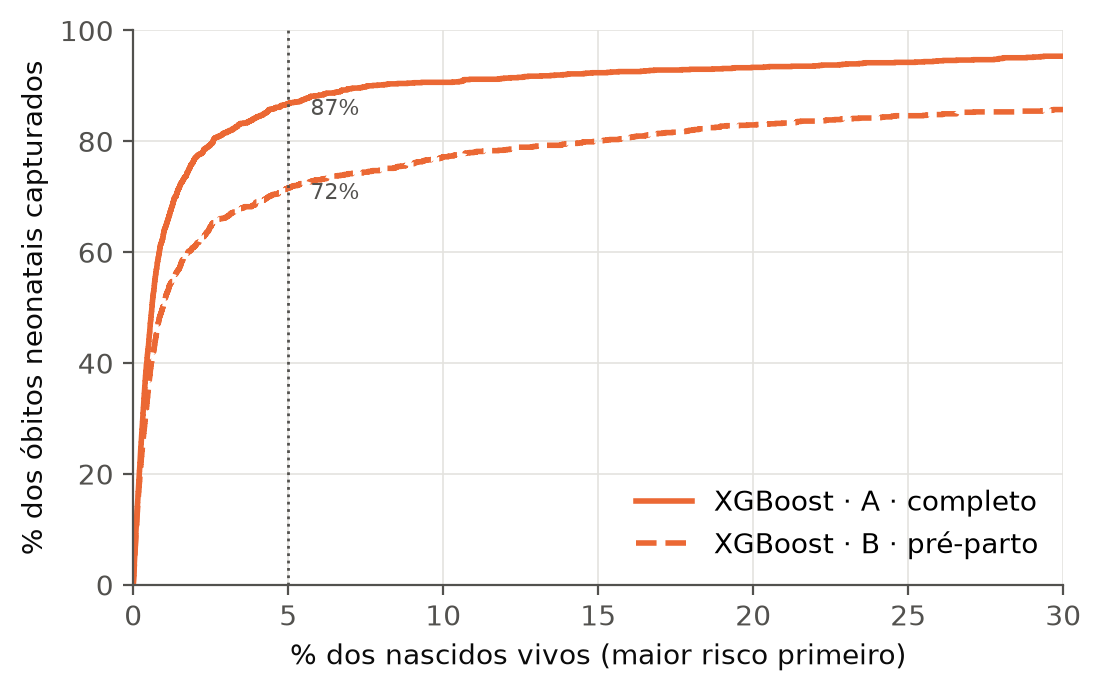
\includegraphics[width=0.6\textwidth]{captura_top.png}
\caption{Fração dos óbitos capturados ao priorizar os nascimentos de maior risco (XGBoost, teste de 2023).}
\label{fig:captura}
\end{figure}

\begin{figure}[ht]
\centering
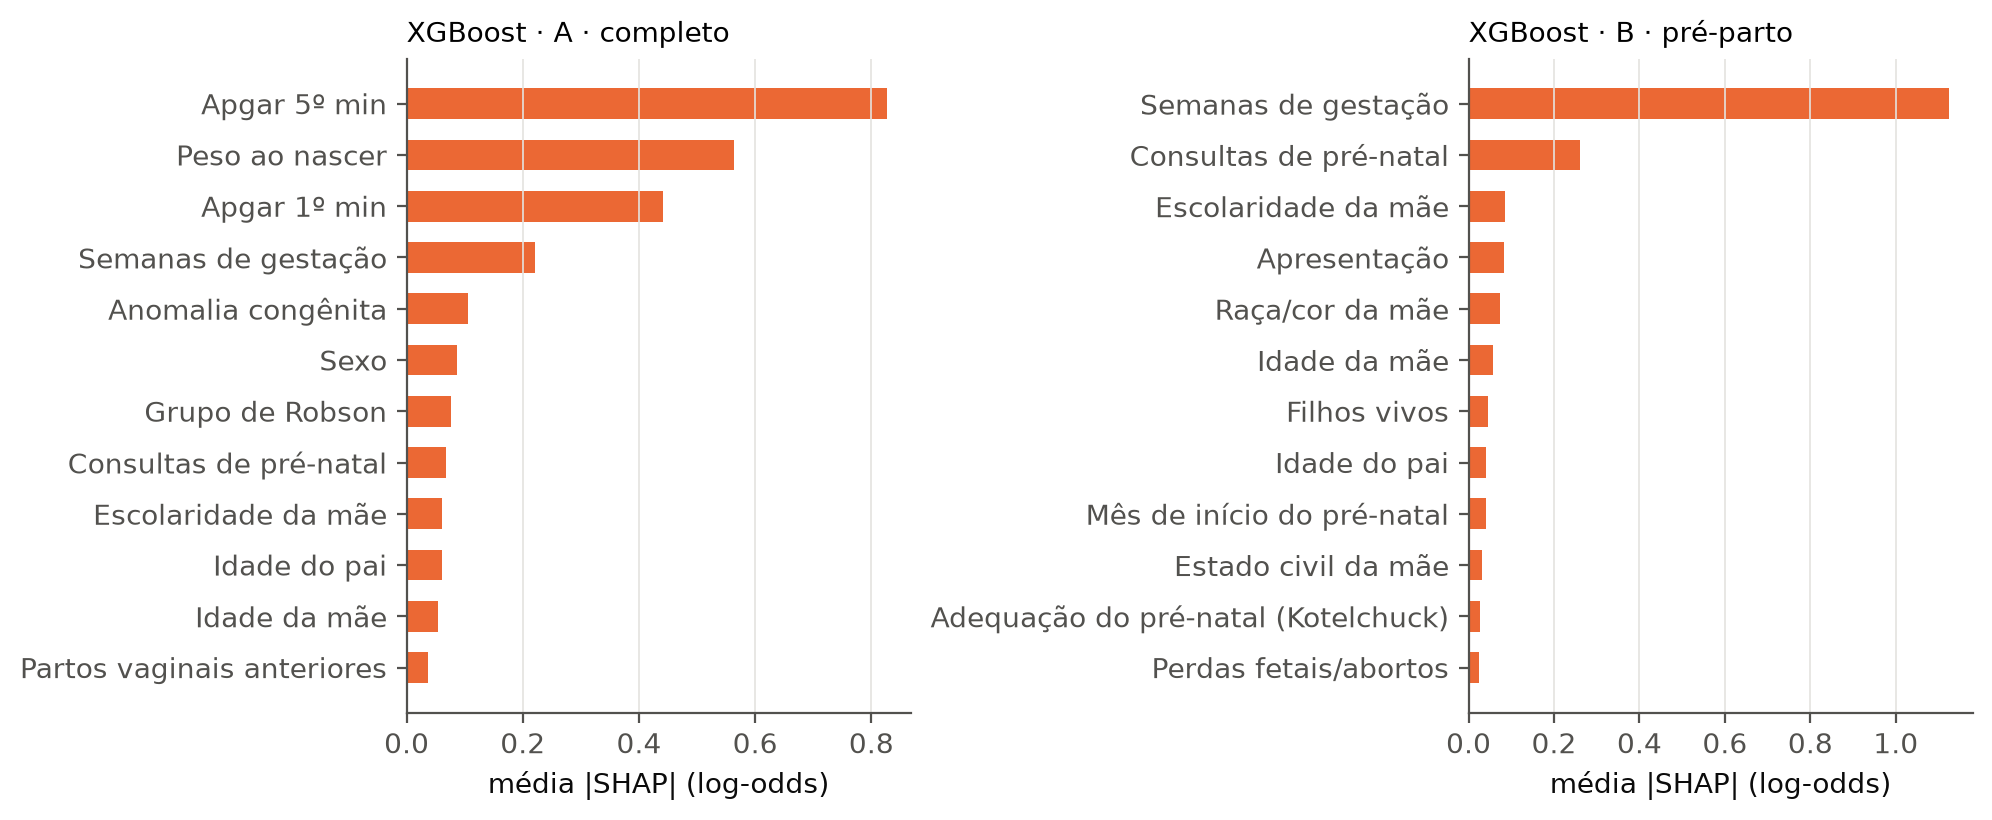
\includegraphics[width=\textwidth]{shap_importancia.png}
\caption{Importância média |SHAP| das 12 principais variáveis (XGBoost, 20.000 nascimentos de 2023).}
\label{fig:shap}
\end{figure}

\subsection{Calibração e subgrupos}

Após a recalibração, a razão O/E no teste foi de \AXgbOE{} (A) e \BXgbOE{} (B). O Brier foi de \AXgbBrier{} e \BXgbBrier{}. O modelo sem recalibração já era bem calibrado (O/E \oeBrutoA{} e \oeBrutoB{}), porque a busca escolheu não reponderar as classes (Figura~\ref{fig:cal}).

Entre os subgrupos (Figura~\ref{fig:sub}), a AUROC do modelo completo variou de \subAAurocMin{} a \subAAurocMax{}, com intervalos de confiança sobrepostos. No modelo pré-parto:
\begin{itemize}
  \item a AUROC foi menor para mães com fundamental incompleto ou menos, \subBFundAuroc{}, do que com superior, \subBSupAuroc{}, mas os intervalos se sobrepõem;
  \item o risco foi subestimado para filhos de mães brancas, com O/E de \subBBrancaOE{};
  \item o risco também foi subestimado para residentes no interior, com O/E de \subBIntOE{}.
\end{itemize}

\begin{figure}[ht]
\centering
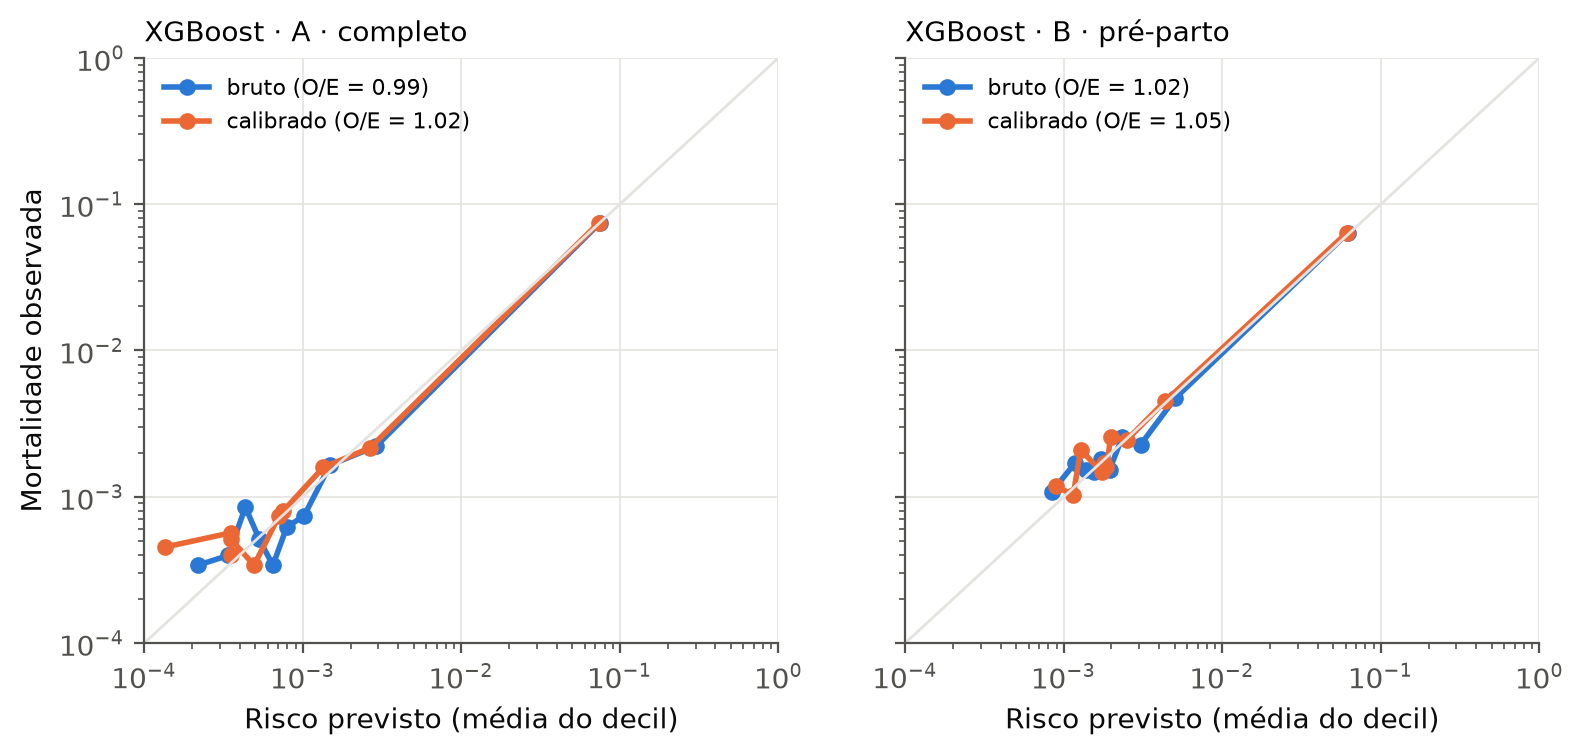
\includegraphics[width=0.9\textwidth]{calibracao.png}
\caption{Mortalidade observada $\times$ risco previsto por decil de risco no teste de 2023, antes e depois da recalibração isotônica (escala logarítmica).}
\label{fig:cal}
\end{figure}

\begin{figure}[ht]
\centering
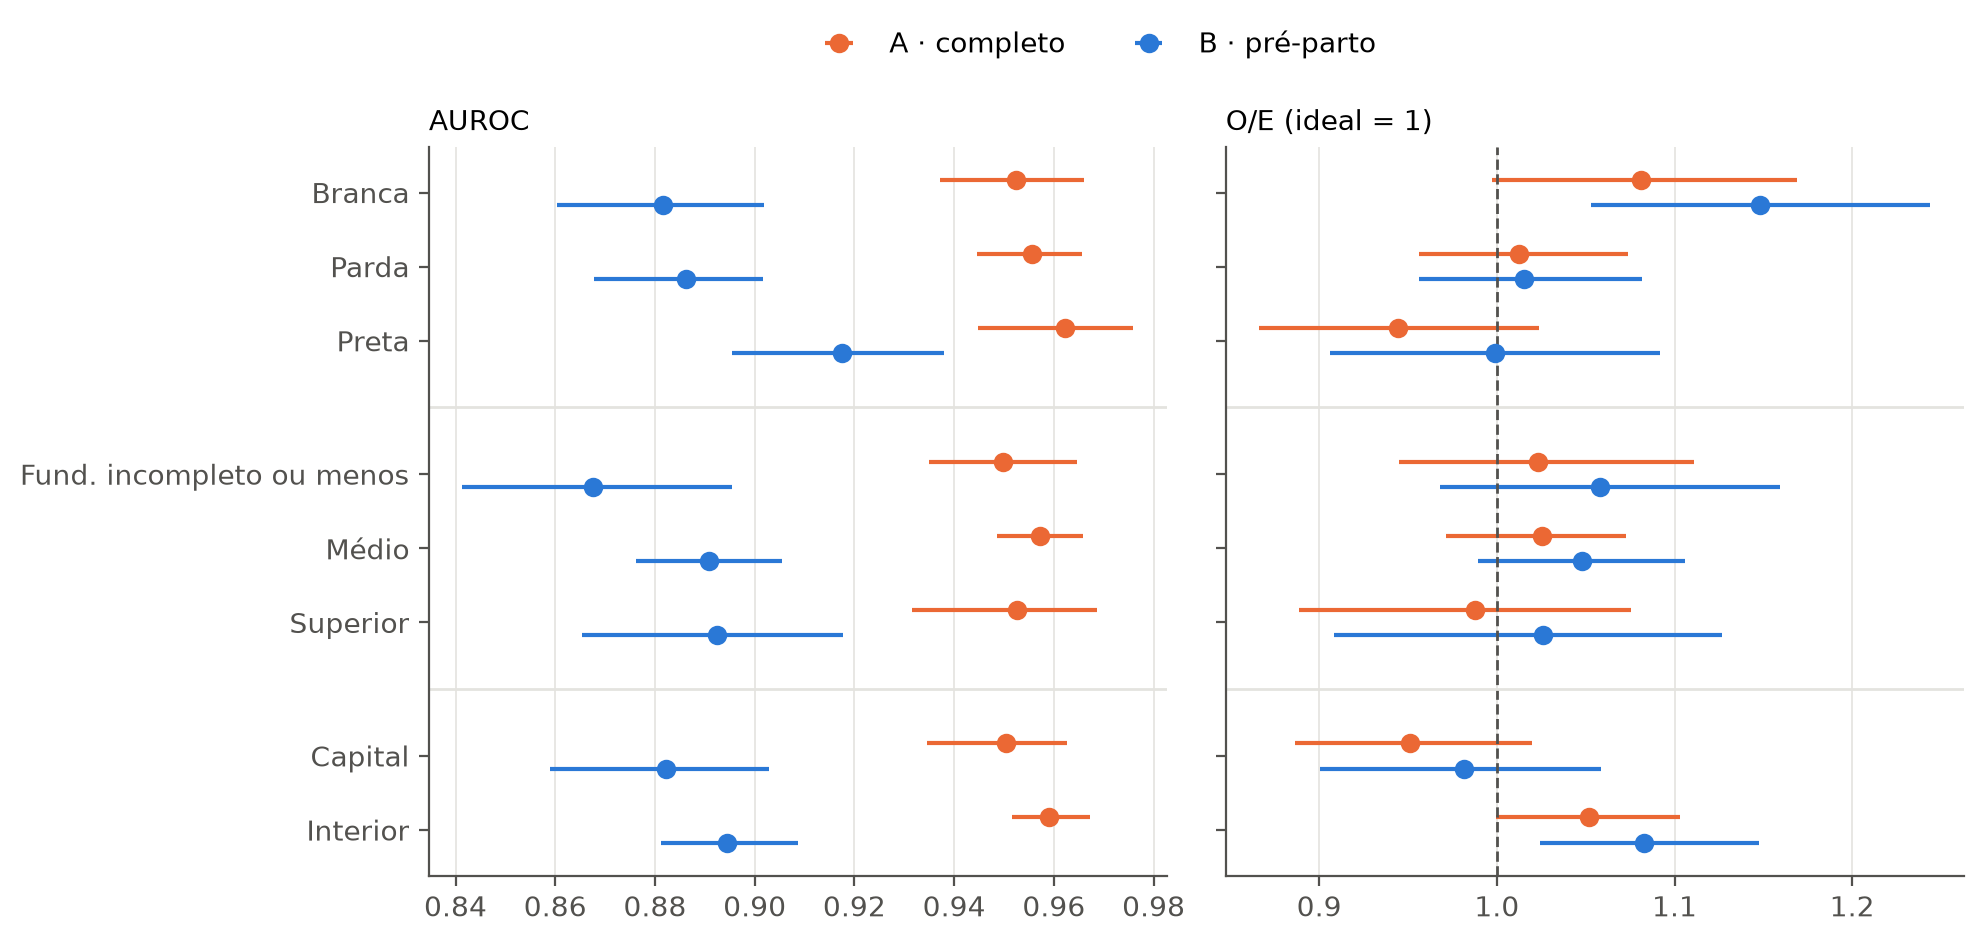
\includegraphics[width=\textwidth]{subgrupos.png}
\caption{AUROC e razão O/E do XGBoost por subgrupo no teste de 2023, com IC 95\% por bootstrap.}
\label{fig:sub}
\end{figure}

\subsection{Sensibilidade ao linkage}

Sem as passadas tolerantes, a AUROC foi de \sensAAuroc{} (A) e \sensBAuroc{} (B), contra \AXgbAuroc{} e \BXgbAuroc{} com todos os pares. A AUPRC foi de \sensAAuprc{} e \sensBAuprc{}.

% ---------------------------------------------------------------------------
\section{Discussão}

\textbf{H1 (reprodução).} O resultado confirma a hipótese. Com dados abertos e linkage sem identificadores, o XGBoost atingiu AUROC de \AXgbAuroc{} e concentrou \AXgbTop{} dos óbitos nos 5\% de maior risco, próximo dos valores do artigo (0,971 e mais de 90\%). As cinco principais variáveis também foram as mesmas.

A diferença residual tem três explicações plausíveis, que não se excluem:
\begin{itemize}
  \item o pareamento de \pctPareado{}: os óbitos não pareados ficam rotulados como sobreviventes;
  \item a população estadual é mais heterogênea do que a de um único município;
  \item a qualidade de preenchimento da DN varia entre os municípios do interior.
\end{itemize}

No limiar escolhido em 2022, a sensibilidade é maior e a precisão menor do que no artigo. Essa diferença decorre da escolha do limiar, e não do modelo.

\textbf{H2 (pré-parto).} A hipótese se confirma só em parte. A perda foi real ($\Delta$AUROC = \dAB{}) e grande em AUPRC, mas o modelo pré-parto ficou acima do esperado, com AUROC de \BXgbAuroc{}. Priorizando 5\% das gestantes na admissão, ele captaria \BXgbTop{} dos óbitos neonatais, quase todo esse poder vindo da idade gestacional e do pré-natal.

Há uma ressalva: usamos a idade gestacional registrada no parto, que é uma aproximação da estimativa disponível na admissão. Na prática, esse modelo serviria à regulação de gestantes de alto risco para maternidades com UTI neonatal, e não ao cuidado depois do nascimento.

\textbf{H3 (calibração e equidade).} A hipótese tem apoio fraco. O modelo completo tem calibração e discriminação homogêneas entre os subgrupos. No pré-parto, a AUROC é numericamente menor na baixa escolaridade, mas os intervalos se sobrepõem. A subestimação para filhos de mães brancas e para o interior sugere que variáveis socioeconômicas e regionais carregam, nesse modelo, parte do risco que no modelo completo é explicado pelo estado do recém-nascido.

\textbf{Limitações.}
\begin{itemize}
  \item Cerca de 10\% dos óbitos não foram pareados, e os falsos pares introduzem ruído no rótulo. A análise de sensibilidade indica, porém, que o ruído não altera as conclusões.
  \item A validação é temporal, mas não externa, porque usa um único estado.
  \item O desempenho alto do modelo completo vem de variáveis medidas depois do nascimento, então ele identifica recém-nascidos já graves, e não uma chance de prevenção antes do parto.
  \item Os subgrupos amarelo e indígena não tiveram óbitos suficientes para análise.
\end{itemize}

% ---------------------------------------------------------------------------
\section{Conclusão}

É possível reproduzir, com dados totalmente abertos, um modelo brasileiro de predição de mortalidade neonatal com desempenho próximo ao publicado. O linkage por chaves compostas pareou \pctPareado{} dos óbitos, taxa comparável à de dados identificados, e pode ser reaplicado a qualquer UF. Um modelo restrito à admissão para o parto mantém AUROC de \BXgbAuroc{} e boa calibração.

Como trabalhos futuros:
\begin{itemize}
  \item validação externa em outras UFs;
  \item etapa probabilística no linkage para recuperar os óbitos não pareados;
  \item extensão ao óbito pós-neonatal;
  \item idade gestacional estimada no pré-natal;
  \item avaliação do uso do escore junto a gestores da rede de atenção materno-infantil.
\end{itemize}

\textbf{Reprodutibilidade.} O código (download, linkage, pré-processamento, modelos, avaliação), os testes, o notebook e os geradores deste relatório e dos slides estão no repositório do projeto. O comando \texttt{python -m src.experimento} refaz todos os números a partir do FTP do DATASUS.

\bibliographystyle{sbc}
\bibliography{refs}

\end{document}
